\lchapter[case]{Case study}

\section{Introduction}

\p{A custom application}
As introduced in the previous chapter, complex systems can be modeled using multi-domain graphs. By using this model, we can then exploit the wide range of already existing tools to manipulate, analyze and visualize generic graphs. As we will see, specific support for multi-domain graphs is almost nonexistent in the network tools ecosystem and we decided thus to develop our own multi-domain graph visualization application.

\p{State of the art}
Before beginning the design of the application, we analyze the current state of the art, by comparing the features of different graph visualization softwares with regard to multi-domain graphs layout and visualization. This analysis of the state of the art is covered in \vref{sec:case/art}.

\p{Architecture}
After having made an overview of what the different applications and utilities present in the ecosystem are capable of, we can define a first sketch of the architecture of the application we are going to develop. This overview is presented in \vref{sec:case/arch}.

\p{Technologies}
As last point, before beginning the software development life cycle, we define the technologies we are going to use with regard to the points emerged in both the research about the state of the art and the definition of the overall architecture. This argument is covered in \vref{sec:case/tech}.

\section{State of the art}
\label{sec:case/art}

\p{Overview}
For the purposes of the analysis of the state of the art, we focus our research on three major graph/network analysis and visualization applications: Pajek \cite{pajek}, Gephi \cite{gephi}, and Cytoscape \cite{cytoscape}. We evaluate each ``candidate'' against the following criteria:

\begin{description}
  \item[Programming language] The programming language used to develop the application. If an application is closed source this criterion is mostly irrelevant.
  \item[Execution environment] The environment that the application supports and its specifics. An environment could be ``Desktop'' and the specifics ``Windows XP and later''.
  \item[User experience] A totally arbitrary and personal evaluation of the ease of use and the general user experience when using the application.
\item[\gls{3d} rendering] Whether or not an applications supports visualization of graphs in \gls{3d} space.
  \item[Explicit multi-domain support] Multi-domain graphs support as an explicit feature (i.e., stated as such).
  \item[Emulated multi-domain support] Multi-domain graphs support achieved by ``hacking'' on other features (e.g., hierarchical graphs).
  \item[Supported file formats] An enumeration of the supported input and output file formats, as well as other means to push data to or get it from the application.
\end{description}

\p{Results overview}
A summary of the results of the analysis is reported in \vref{tab:usecase}. The next three subsections, instead, contain the detailed discussion of the analysis of each application.

\begin{table}
  \begin{threeparttable}
    \rowcolors{2}{white}{gray!10}
  \begin{tabularx}{\textwidth}{ >{\small\raggedleft\arraybackslash} m{3.28cm} | >{\footnotesize\centering\arraybackslash} m{3cm} | >{\footnotesize\centering\arraybackslash} m{3cm} | >{\footnotesize\centering\arraybackslash} m{3cm} }
    \toprule
    & \normalsize{Pajek} & \normalsize{Gephi} & \normalsize{Cytoscape} \\
    \hline

      Programming language & C & Java & Java \\
      Execution environment & Desktop (Windows) & Desktop (Java VM) & Desktop (Java VM) \\
      User experience & 3/10 & 7/10 & 8/10 \\
      \gls{3d} rendering & No & Yes\tnote{1} & Plugin (not working) \\
      Explicit multi-domain support & No & No  & No \\
      Emulated multi-domain support & No & Partial (5/10) & Partial (6/10) \\
      Supported file formats & NET, DL, GraphML (export only) & GML, NET (import only), GraphML, GEXF, CSV, DL, \ldots & SIF, NNF, GML, XGMML, CSV, GraphML, \ldots\tnote{2}\\

    \bottomrule
  \end{tabularx}
  \vspace{1mm}
  \begin{tablenotes}
  \item [1] \footnotesize{Supported by the rendering engine, but no functionality exposed by the \gls{ui}.}
  \item [2] \footnotesize{However, the importing process failed in all our tests.}
  \end{tablenotes}
  \end{threeparttable}
  
  \caption[Summary of the analysis of three graph visualization applications.]{Summary of the analysis of three graph visualization applications: Pajek, Gephi, and Cytoscape. The notation scale and the assigned value is completely arbitrary and shall just serve as rough indication of the state of a particular feature.}
  \label{tab:usecase}

\end{table}


\subsection{Pajek}

\p{Overview}
The first application we study is called \emph{Pajek} \cite{pajek} and is heavily orientated towards network analysis. Although it includes some visualization features, they are intended as output channel and only allow very limited interactivity. The main advantage of Pajek is its extensive academic background, also reflected by the community backing it.

\p{Environment and platform}
Pajek is a stand-alone software freely available for non commercial uses and runs under Windows. It is written in C and offers relatively good performances being able to handle graph in the order of \numprint{500000} nodes \cite{compa}.

\p{User experience}
The legacy of Pajek is very apparent in its user interface (cf. \vref{fig:pajek}). The user experience follows suit with a non-intuitive interface and very few visual hints. No guidance is provided at all to the end user.

\begin{figure}
  \centering
  \includegraphics[width=.8\linewidth]{images/pajek}
  \caption[Screen shot of Pajek.]{Screen shot of the \emph{Pajek} network analysis application.}
  \label{fig:pajek}
\end{figure}

\p{Multi-domain support}
Pajek can analyze very large networks and has some tools to work with hierarchical graphs, but it does not have any explicit support for multi-domain network analysis. Additionally, given the limited visualization capabilities, it is probably not a good candidate to solve the problem at hand.

\p{Formats}
The main graph format supported by Pajek is its own \emph{NET} format. While this format is well supported across other graph manipulation and visualization tools, it is not very well documented nor does it support necessary features such as node/edge attributes. GraphML is supported as an export-only format \cite{compa,net,pajekman}.

\p{Summary}
The analysis-oriented approach that Pajek offers to its users does not allow us to generate interactive visualizations. Additionally, its legacy software architecture does not lend itself well to be extended with custom plugins. We can surely learn a lot from the analysis tools provided by it, but Pajek is probably not a good base to use to visualize multi-domain graphs.

\subsection{Gephi}

\p{Overview}
The second candidate of the case study is \emph{Gephi} \cite{gephi}, a newcomer to the graph visualization scene (the first commit in the public repository is from March 2009) but which has already built a great community and ecosystem. Gephi is oriented towards graph visualization, but includes powerful analysis tools as well.

\p{Environment and platform}
Gephi is an open-source Java desktop application and as such supports all major operating systems (Windows, OS X, and Linux). Its architecture is extremely extensive and plugins can be developed to tune almost any part of the system (e.g., layout algorithms, filters, clustering algorithms, metrics, \ldots).

\p{User experience}
The user interface presented by Gephi is very intuitive and, at first glance, user friendly. Sadly, after some more intense work, many feature still seem incomplete or do not work as expected. Despite still being in its infancy, Gephi has already done a good work in the area of user experience.

\begin{figure}
  \centering
  \includegraphics[width=.8\linewidth]{images/gephi}
  \caption[Screen shot of Gephi.]{Screen shot of the \emph{Gephi} graph visualization application.}
  \label{fig:gephi}
\end{figure}

\p{Visualization capabilities}
Gephi's main feature are its interactive visualization tools. It supports iterative layout algorithms continuously modifying the graph and provides different tools to work on the visualization in real-time (i.e., no rendering phase is necessary). It sill lacks more advanced tools (such as edge bundling) and many of its limitations regarding the visualization derive from the overly simplistic graphics primitive used: currently just circles connected by straight lines. Basic \gls{3d} support is provided by the underlying rendering engine, but none of those features are exposed in the user interface.

\p{Multi-domain support}
Multi-domain graphs are not supported by Gephi at all. While it supports hierarchical graphs, the application is not yet ready to handle them in a meaningful way, mainly because of the missing \gls{ui} controls.

\p{Formats}
One area in which Gephi really shines is when working with different data sets. It has extensive support for importing and exporting from/to different formats, and additional ones can be added by means of the plugin architecture. Additionally, Gephi also exposes a networking interface to act both as a client or as a server to stream graphs over the network.

\p{Summary}
Gephi could be a good candidate to be used as a base for an application to visualize complex systems modeled as multi-domain graphs, but we would probably be spending more time fixing parts of the application which still are not complete rather than focusing on the core problem.


\subsection{Cytoscape}

\p{Overview}
The last application we evaluate as part of this study is called \emph{Cytoscape} \cite{cytoscape}. Initially made public in July 2002, Cytoscape is an open-source software platform originally conceived for visualizing molecular interaction networks and biological pathways. Nowadays, Cytoscape, provides functionalities to analyze and visualize arbitrary networks.

\p{Environment and platform}
So as Gephi, also Cytoscape is a desktop application written in Java and running under all major operating systems. It provides extension points for plugins, called \emph{Apps}, to customize most parts of the application.

\p{User experience}
From all tested softwares, Cytoscape is the one with the most care put into the user interface. Different tools are readily available and easy to use, but it is still noticeable that this tool is intended for scientists that already know the domain. A negative note goes is the low interactivity supported by the visualizations. For example, layout algorithms are applied synchronously: while the layout is calculated nothing moves and the user has to wait for a progress bar to complete.

\begin{figure}
  \centering
  \includegraphics[width=.8\linewidth]{images/cytoscape}
  \caption[Screen shot of Cytoscape.]{Screen shot of the \emph{Cytoscape} graph analysis and visualization application.}
  \label{fig:cytoscape}
\end{figure}

\p{Visualization capabilities}
The visualization capabilities provided by Cytoscape are unmatched in the other tested softwares. The quality of the renderings is very good and different tools help to make it even better. One example among all is the support for edge bundling (and thus curved paths with multiple handles). No built-in \gls{3d} support is available and the plugin which should add it failed to install (its last release is from 2011, so it may not be up to date anymore).

\p{Multi-domain support}
While no explicit multi-domain graphs support is provided by Cytoscape, the range of available tools makes it the best candidate to emulate multi-domain visualizations.

\p{Formats}
Cytoscape offers import and export functionalities for different formats, sadly we were not able to import any test file (Pajek NET, Gephi exported formats, GraphML, \ldots) and had to recur to a data set found on the web for the visualization tests.

\p{Summary}
Cytoscape surely is a mature software with good foundations (even if some aspects could still be polished, cf. Formats) and powerful tools. Its user interface is good but suffers from the cluttering due to the widgets needed to support the many offered functionalities. The good quality of the visualization sometimes also impacts the rendering performances.

\section{Web application}

\subsection{Introduction}

\p{Reasons}
The applications presented in the previous section all provide useful features to work on graphs. As we saw, none of them supports multi-domain graphs out of the box, but support for them could eventually be added through the use of plugins or direct modifications to the source code. The best candidate to be extended to support multi-domain graphs would be Cytoscape. However, for different reasons, we choose to develop our own web-based application.

\p{Entry barrier}
Beside the challenge of developing an application handling graphs with thousand of nodes running in a browser, and the academic interest in the proof that this particular type of environment can be exploited to execute resource-demanding applications, there are more practical reasons as well. First of all, the entry barrier is much lower: instead of downloading and installing an application weighing in the hundreds of megabytes, the user simply has to open a link.\footnote{Interesting fact: we tested the final version of the application on a Samsung S4 device in the standard Chrome browser and we were able to display some basic graphs. Clearly the performances were not satisfying, but this indicates that it might be possible to expand the application to support mobile devices in the future.} The same applies to updates, as they are instantly deployed to all users.

\p{Performance}
While remaining on a single node, a desktop application can be much more performant than a JavaScript based one, but to scale beyond a certain point the work has to eventually be distributed across different nodes. By developing an application that is inherently distributed, adding an additional tier for, e.g., layout computation, becomes a natural evolution.

\p{Collaborative}
An additional reason is the collaboration possibilities that a web based platform enables. In the same way as layout computation may be distributed across multiple nodes, different users may collaborate on the same by acting on the same graph.

\p{Structure of the section}
In the remaining parts of the present section we first discuss the overall system architecture to cope with the main features we need to support (\vref*{sec:case/arch}) and then present the technologies on which we choose to base our application on (\vref*{sec:case/tech}).

\subsection{Overall system architecture}
\label{sec:case/arch}

\p{From tasks to components}
The application can be structured into three main components derived directly from the tasks it will be used for, as discussed in \ref{sec:intro/collection} and \vref{sec:intro/visu}, and summarized in the following list:

\begin{enumerate}[itemsep=-2pt]
    \item Data collection: The first task is the collection and aggregation of data from different sources. Examples of data sources are mailing lists, version control repositories (historical data), source code, issue trackers, etc.
    \item Data analysis: Once all data is collected and stored in a standardized format, different metrics and analysis tools can be run on it to produce additional insights and comparison methods.
    \item Data visualization: The last task, is to take all the results and present them in a meaningful way to the user. Data will be visualized as a graph, but other visualization approaches can be imagined (e.g., Design Structure Matrices \cite{dsm}). Additionally, it should be possible to extract metrics and other statistical insights from the data at hand.
\end{enumerate}

\begin{noteframe}[frametitle={Note}]
The second point in the list above, the data analysis task, was initially planned but then removed from the initial version of the toolkit in order to focus more on the visualization aspects. For the purpose of this chapter, we assume that it will be included in the final architecture.
\end{noteframe}
  
\p{Extensibility}
As data can come from a plethora of different sources, as the employed visualization techniques may not be adapted to a certain domain, and as the analysis possibilities are endless, it is impossible for the toolkit to cover all possible applications. To obviate to this problem, the design has to account for a completely pluggable architecture, in which new data collectors, visualization engines, and analysis tools can easily be added and removed as the need arises.

\p{Architecture}
From an architectural point of view, having chosen to develop the application as a web application already forces us to adopt at least a 2-tier architecture: a back-end for the heavy lifting and a rich-thin client as front-end. As the data collection process can eventually require a considerable amount of resources, we delegate this task to an additional tier, called the acquisition server. The component diagram in \vref{fig:comp-app} shows this architecture graphically. Even if the decision could be taken at a later point in time, we have already decided that, to account for pluggable data collectors and scalability, the acquisition server will be a 2-tier service by itself, bringing the total number of tier of the application up to 4.

\p{A note about databases}
The astute reader may have noticed that one tier is absent from the presented architecture: a database. While a database is effectively needed for the normal operation\footnote{We consider \emph{normal operation} activities such as authentication/authorization, configuration management, and other processes not directly related to the core functionality.} of the web application back-end, for the purposes of this analysis, we consider it an implementation detail. On the other hand, an additional datastore is needed to store the graphs resulting from the different data collection processes. While a specialized graph database was initially planned, it was later discarded as overkill for the current state of the application. Adding a databases and being able to exploit it efficiently and effectively would in fact introduce too many dependencies between otherwise decoupled modules. Note that we do not have discarded the idea completely, but we simply assert that is not the most important feature to provide support for at this stage of the development.

\begin{figure}
  \begin{adjustwidth}{-0.3mm}{-0.7mm}
	  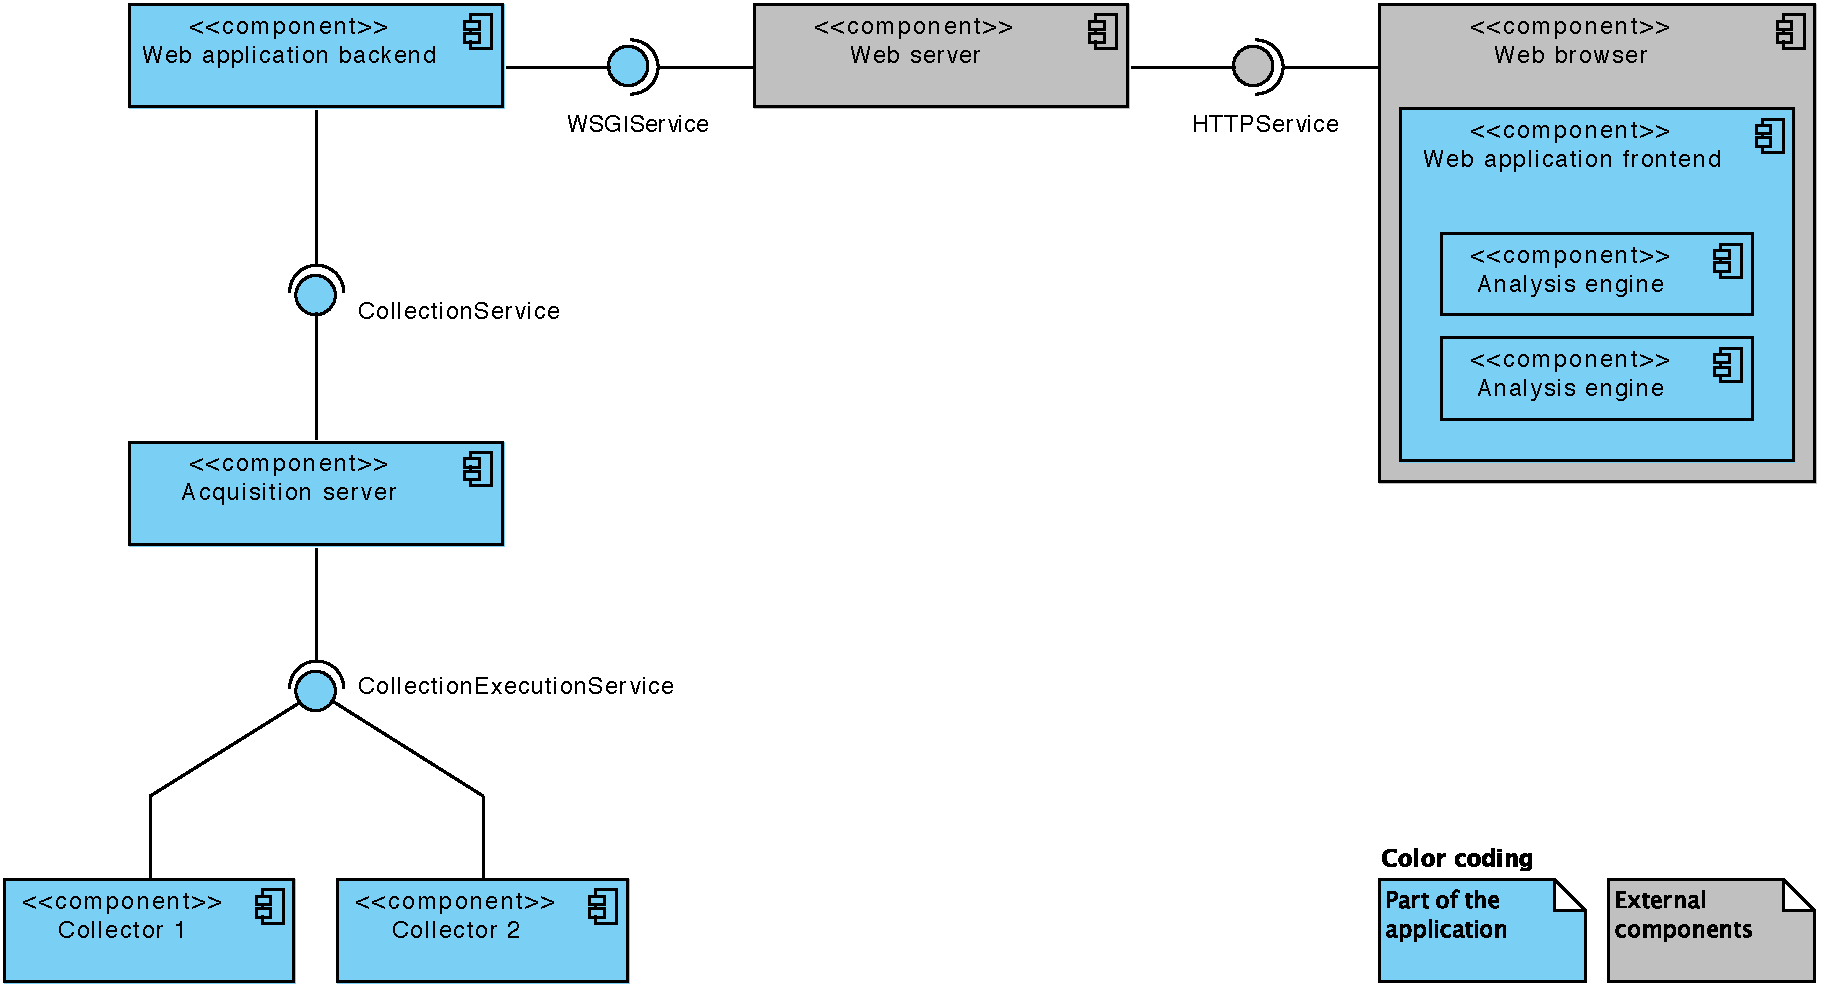
\includegraphics[width=\linewidth]{comp-app}
  \end{adjustwidth}
	\caption[Architectural overview of the \gls{csat} software suite.]{Overview of the \gls{csat} suite illustrating the 4-tier architecture}
	\label{fig:comp-app}
\end{figure}

\p{Scalability}
The 4-tier architecture presented in the previous paragraph allows to account for different degrees of scalability in the data acquisition process. The process can in fact be scaled horizontally by distributing the \emph{Collector} components across different systems.

\subsection{Selected technologies}
\label{sec:case/tech}

\p{Introduction}
Given the 4-tier architecture presented in the previous subsection, we can already define the different technologies we will use to implement the different components. While the web application back-end, the acquisition server and the collectors can all run in the same environment, the front-end is running in a web browser. As a consequence, we will have at least two different technology stacks.

\p{Back-end and acquisition server}
We choose to use Python \cite{python} as the programming language for the back-end, mainly because it is the language we know the best and because of the wide range of available libraries to work on graphs. On top of Python, we use Django \cite{django} as web framework for the web application back-end and Twisted \cite{twisted} as networking framework for the acquisition server. The collectors implemented as part of this project are written in Python as well, but any programming language can be used as long as the correct interface is implemented.

\p{Front-end}
The choice of the programming language for the front-end is easier: if we want to avoid plugins and rely on native browser support, we have to use JavaScript. To help with the development, we use CoffeeScript \cite{coffee}, a small language that compiles to JavaScript but removes some of its quirks. To render the graphs we use WebGL \cite{webgl}, a relatively new technology which provides an \gls{api} similar to OpenGL \cite{opengl} to access the \gls{gpu} for \gls{3d} graphics from JavaScript. We access the WebGL \gls{api} using the abstraction layer provided by THREE.js \cite{three}.

\p{Data format}
The graphs will be stored in GraphML \cite{graphml}, a well established format supported by all the tested applications. GraphML is based on \gls{xml} and can be extended with custom elements to fit our needs. Out of the box it supports directed, undirected and mixed graphs, nodes and edges data, hierarchical graphs, hypergraphs, etc.

\subsection{Multi-domain graph format}

\p{Introduction}
In the previous section we stated that we will use GraphML as the format of choice for the graphs handled by the application. Neither GraphML nor any other graph format handles multi-domain data natively, but we can save a multi-domain graph structure as a normal graph by following a given convention.

\p{Format convention}
A GraphML file can contain one or more graphs and supports hierarchical graphs. This means that graphs can be nested (\ie a node can contain a whole subgraph) and links can be defined to/from nodes in a graph and in a subgraph. For the purposes of our application, we need to identify the domains to which the nodes of a graph belong to, we can achieve our goals with the following convention:

\begin{quote}
Each domain is modeled using a subgraph which lives in a single node of its single parent graph element. This is equivalent to saying that each document contains a single graph. This graph contains a node for each domain it models. Each domain-node contains a subgraph (or nested graph) which in turn contains the nodes of the elements in the specific domains. In case of single-domain documents, the parent graph will always be present. Each graph shall expose information about the domains it models.
\end{quote}

More details about the GraphML format and how it is used to model multi-domain graphs can be found in \vref{sec:acquisition/implementation/merging}.
